\documentclass[a4paper,12pt]{article}

\usepackage[utf8]{inputenc}
\usepackage{polski}
\usepackage{a4wide}

\usepackage[colorlinks=true,linkcolor=blue,urlcolor=blue]{hyperref}

\usepackage[pdftex]{graphicx}



\hypersetup{
	unicode = true,
	pdfauthor = {Jakub Kotur},
}

\title{OpenStack Storage (Swift)}
\author{Jakub Kotur}

\hyphenation{IaaS Rack-Space}

\begin{document}
\maketitle

\section{Wstęp}

\nocite{openstack}

OpenStack Storage, inaczej nazywany Swift, jest systemem chmurowym pozwalającym na przechowywanie danych. Długo obiekty które są przechowywane przez system miały ograniczenie wielkości 5GB, jednak niedawno twórcom udało się z nim poradzić. Swift pozwala na przechowywanie płaskiej struktury obiektów (plików), grupowanych w kontenerach. Każdy użytkownik może posiadać dowolnie dużo kontenerów,~a w nich dowolnie dużo plików. W zależności od konfiguracji system pozwala na tworzenie kopii zapasowych, oraz automatyczne zarządzanie tymi kopiami. API systemu oparte jest na prostych wywołaniach PUT, GET oraz paru innych. Swift pozwala również na użycie dowolnego systemu autoryzacji, jednak twórcy dostarczają gotowe rozwiązanie, które wspiera zarówno standardowe podejście użytkownik:grupa, jak i ACL.

%\section{Możliwości}\label{sec:możliwości}

%\section{Zastosowania}\label{sec:zastosowania}

\section{Architektura}\label{sec:architektura}

W poniższym rozdziale opisana zostanie architektura Swifta. Jest to bardzo poglądowe podejście do tego co i jak się dzieje, aby zapewnić poprawne działanie systemu. Swift jest złożonym systemem w którego skład wchodzą zarówno usługi serwerowe, jak i procesy odpowiedzialne za utrzymanie spójności danych. Praktycznie każdy z tych komponentów można uruchomić na dowolnej ilości oddzielnych maszyn, tak aby zapewnić możliwie dużą niezawodność chmury.

\subsection{Główne komponenty}\label{sub:glowne komponenty}

\subsubsection{Serwery}\label{sub:serwery}

\begin{description}
\item[Serwer proxy] (Proxy Server) -- serwer odpowiedzialny za kontrolę nad innymi serwerami chmury. Do niego wysyłane są zapytanie API, które następnie kieruje do odpowiednich serwerów. Jest również odpowiedzialny za kontrolę błędów, np. jeśli okaże się że wywołany serwer jest niedostępny, to właśnie serwer proxy znajduje jego serwer lustrzany i wysyła nowe zapytanie.
\item[Serwer obiektów] (Object Server) -- prosty serwer przechowujący pliki jako dane binarne. Dodatkowe metadane o plikach przechowywane są w rozszerzonych atrybutach plików. W zależności od ustawień może być replikowany, tak że kilka serwerów przechowuje takie same dane.
\item[Serwer kontenerów] (Container Server) -- bardzo podobny do serwera obiektów, jednak przechowujący informacje o tym co znajduje się wa danym kontenerze. Dane przechowywane są w bazie SQLite jako szereg wpisów z nazwami obiektów. Analogicznie do serwera obiektów można tworzyć repliki tych serwerów.
\item[Serwer kont] (Account Server) -- identyczny z serwerem kontenerów, tylko przechowuje dane o kontenerach które posiada dane konto.
\end{description}

Serwery obiektów, kontenerów i kont, nazywane one będą od tej pory wspólnie serwerami danych. Jest to o tyle uzasadnione, że są one do siebie na tyle podobne, że większość procesów i zachowań jest wspólna. Serwery kont i kontenerów są wręcz, z punktu widzenia sposobu przechowywania danych, identyczne.

W powyższym zestawieniu nie został w żaden sposób uwzględniony serwer autoryzacji. Co prawda Swift udostępnia swoje rozwiązanie, jednak można w to miejsce wstawić dowolne inne rozwiązanie. Twórcy OpenStacka uznali więc, że autoryzacja jest zupełnie odrębna od Swifta.

\subsubsection{Procesy}\label{sub:procesy}

Poniżej wymienione procesy odpowiedzialne są za utrzymywanie poprawnych i spójnych danych w chmurze. Wszystkie one chodzą lokalnie na serwerach danych, i jeśli natrafią na jakiś problem, starają się go rozwiązać komunikując się z innymi serwerami.

\begin{description}
\item[Aktualizatory] (Updaters) -- procesy dbający o to, aby aktualizować dane na serwerach. Jeśli z jakiegoś powodu aktualizacja danych do serwera nie zostanie wysłana, albo przez serwer odebrana, zostaje ona zakolejkowana. Po z góry ustalonym czasie próba aktualizacji jest ponawiana.
\item[Audytory] (Auditors) -- procesy sprawdzający poprawność danych lokalnych. Jeśli napotka zepsuty plik, stara się go naprawić ściągając z innej repliki. Jeśli naprawa jest niemożliwa, błąd jest logowany. 
\item[Replikatory] (Replicators) -- również dbają o spójność danych, jednak ich zadaniem jest utrzymywanie jednakowej wersji na wszystkich serwerach. Jeśli któryś z serwerów nie ma najnowszej wersji, jego dane aktualizowane są do niej.
\item[Żniwiary] (The Account Reaper) -- albo ładniej, żniwiarz użytkowników, jest procesem który dba o usuwanie danych, które należały do użytkowników usuniętych z systemu. Jeśli uda mu się usunąć wszystkie pliki, oraz kontenery użytkownika, kasuje tego użytkownika z bazy.
\end{description}

\subsubsection{Struktury danych}\label{sub:struktury danych}

\begin{description}
\item[Pierścień] (The Ring) -- jeden z ważniejszych modułów Swifta. Jest to zestaw mapowań z kluczy obiektów Swifta na fizyczne urządzenia. Dzięki pierścieniowi serwer proxy wie do którego serwera wysłać zapytanie. Istnieją oddzielne pierścienie dla obiektów, kontenerów i kont, jednak są one identyczne. W pierścieniu można ustawić poziom replikacji serwerów. Również serwery udostępniające pierścienie mogą być powielane.
\item[Urządzenie] (Device) -- lokalizacja fizycznego dysku w chmurze z dodatkowymi danymi na jego temat. Na podstawie danych zawartych w opisie urządzenia pierścień zna dokładne miejsce, co do partycji systemowej, gdzie ma zostać wysłane zapytanie. Może również dynamicznie wybierać lepsze, bądź po prostu aktualnie aktywne urządzenia.
\end{description}

\subsection{Przykładowa konfiguracja}\label{sub:przykladowa konfiguracja}

Na \hyperref[fig:swift_arch]{rysunku \ref{fig:swift_arch}} została przedstawiona najprostsza konfiguracja chmury Swifta. Serwer autoryzacji, oraz serwer proxy muszą być dostępne dla użytkowników, aby mogli oni wysyłać zapytania do chmury. Użytkownik najpierw odpytuje serwer autoryzacji o swój token, następnie cała komunikacja odbywa się za pośrednictwem serwera proxy. Serwery opisane na obrazku jako storage, są wspomnianymi wcześniej serwerami danych. Najwygodniejszą lokalizacją dla pierścienia, jest publiczny serwer proxy. Konfiguracja serwerów danych jest dowolna, dopóki serwer proxy potrafi się z nimi komunikować.

\begin{figure}
\centering
	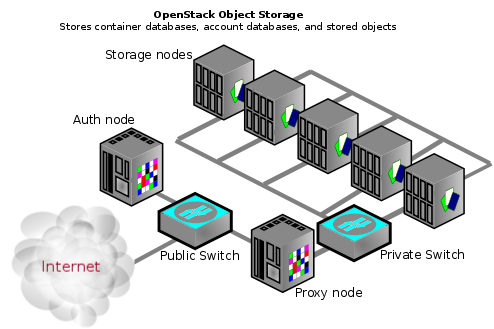
\includegraphics[width=0.75\textwidth]{swift_install_arch.png}
	\caption{Przykladowa architektura swifta~\cite{swift_manual}}
\label{fig:swift_arch}
\end{figure}


\subsection{Replikacja}\label{sec:replikacja}

Replikacja w Swifcie podzielona jest na dwa moduły. Jeden odpowiada za replikację obiektów (danych), drugi za replikację kontenerów i kont, czyli efektywnie baz danych. Oba moduły jednak polegają na zasadzie PUSH, czyli każdy serwer dba o to, aby jego dane lokalne jeśli są nowe, znalazły się na wszystkich replikach. Wysyłanie odbywa się poprzez pierścień, który decyduje które fizyczne serwery są replikami danego serwera. Mechanizm ten wygląda w ten sposób, ponieważ serwer nie wie skąd pobrać dane,~a więc i gdzie są nowsze dane niż te które posiada. Wspomniany zostanie również mechanizm usuwania danych z chmury, który również jest częścią systemu replikacji, ponieważ jest on nieoczywisty. 

Trzeba zaznaczyć że prace nad modułem replikacji w Swifcie są aktualnie w fazie rozwojowej, więc większość informacji zawartej w tym rozdziale może się niedługo zmienić, bądź już jest nieaktualna. Niemniej ogólna idea zapewne pozostanie taka sama.

\subsubsection{Bazy danych}\label{sub:bazy danych}

W pierwszej kolejności serwery baz danych porównują sumy kontrolne baz, jeśli się zgadzają, synchronizacja nie jest potrzebna. W przeciwnym przypadku synchronizowane są brakujące rekordy.

Serwery baz danych przechowują dodatkową bazę synchronizacji. W takiej bazie istnieje informacja, kiedy ostatnio serwer był synchronizowany z którymi bazami. Bazy rozpoznawane są po unikalnych w skali replikacji identyfikatorach. Jeżeli zdalna baza jest starsza, nowe rekordy są wysyłane. Po wysłaniu wszystkich rekordów cała baza synchronizacji wysyłana jest na zdalny serwer. W ten sposób informacja o synchronizacji z innymi bazami, przechodzi na serwer zdalny.

\subsubsection{Obiekty}\label{sub:obiekty}

Na serwerach obiektów również trzymane są sumy kontrolne dla każdego katalogu z danymi. Jeżeli sumy się różnią, dane z danego katalogu są synchronizowane przy pomocy rsync. Po takiej operacji nowe wyliczane są nowe sumy kontrolne na zdalnej maszynie.

\subsubsection{Usuwanie}\label{sub:usuwanie}

Kiedy z serwera obiektów usuwany jest plik, zamiast usunięcia go, stawiany jest specjalny plik, będący znacznikiem usunięcia. Taki plik ma ten sam identyfikator co poprzednie dane, jednak ma nowszą wersję. Dzięki temu proces odpowiedzialny za integralność danych w chmurze rozpropaguje taki znacznik po wszystkich replikach. Znacznik jest usuwany po czasie zwanym oknem spójności, czyli po czasie po którym jesteśmy pewni że dany plik został rozpowszechniony na wszystkie serwery.

\subsection{Autoryzacja}\label{sec:autoryzacja}

Ponieważ autoryzacja w Swifcie ma historyczne zaszłości i jest mocno związana z innymi systemami Rackspace'a, można ją przeprowadzać na kilka sposobów. Może być prowadzona poprzez zupełnie oddzielny system niezależny od Swifta, bądź przez podsystem Swifta nazywany Swauth. Ogólna koncepcja autoryzacji w systemie opiera się na tokenie autoryzacji, który dołączany jest do każdego żądania wysyłanego przez użytkownika. Token taki jest po prostu bliżej nie określonym stringiem. Z punktu widzenia Swifta ważne jest jedynie aby móc go wysłać do systemu autoryzacji i otrzymać odpowiedź, czy token jest poprawny czy nie. Jeśli odpowiedź jest pozytywna, wraz z nią przychodzi informacja o czasie wygaśnięcia autoryzacji w sekundach. Przez ten czas Swift przetrzymuje token jako poprawny. Autoryzacja jest pierwszą czynnością którą musi wykonać użytkownik systemu. Po zalogowaniu się w serwerze autoryzacyjnym, dostanie on token, który musi być dołączony do każdego zapytania do Swifta.

Wbudowany w Swifta system autoryzacji Swauth pozwala dodatkowo na konta administracyjne. Kiedy normalni użytkownicy ograniczeni są do własnych kontenerów, administratorzy mogą operować na danych w całym systemie.

\subsection{Segmentacja}\label{sec:segmentacja}

Jak zostało już wcześniej wspomniane Swift miał swojego czasu ograniczenie na wielkość jednego pliku wynoszącą 5GB. Aktualnie ograniczenie to zostało zniesione, jednak ograniczenie na wielkość jednego pliku pozostaje i jest konfigurowalne. Domyślnie cały czas jest to 5GB. Aby poradzić sobie z tym ograniczeniem twórcy Swifta wprowadzili ideę segmentacji obiektów. Jeden plik dla użytkownika, może być przechowywany w chmurze jako dowolna ilość segmentów. Aby poradzić sobie z segmentacją, wraz z segmentami do Swifta wysyłany jest specjalny plik manifestu w którym przechowywane są informacje w którym kontenerze i z jakim prefiksem przechowywane są segmenty. Wszystkie segmenty muszą być przechowywane w tym samym kontenerze, jednak plik manifestu może być w innym. Dzięki temu obiekty segmentów nie zaśmiecają listingu bazowego kontenera,~a plik manifestu udaje normalny obiekt.

Dodatkową korzyścią płynącą z segmentacji jest współbieżne wysyłanie pliku przez serwery. Jeżeli np. segmenty zostaną rozprowadzone po różnych centrach danych, użytkownik może pobierać duży plik z prędkością sumaryczną oferowaną przez te serwerownie.

\section{Konfiguracja}\label{sec:konfiguracja}

Swift używa do konfiguracji zewnętrznej biblioteki pythona Paste Deploy~\cite{paste_deploy}, który implementuje standard WSGI odnośnie konfiguracji serwerów. Dokładny opis składni plików konfiguracyjnych znajduje się w dokumentacji tejże biblioteki pod adresem \url{http://pythonpaste.org/deploy/#the-config-file}. 

Konfiguracja każdego serwera znajduje się w pliku \texttt{/etc/swift/<server>-server.conf}, gdzie \texttt{server}em może być proxy, object, container bądź account, w zależności który serwer chcemy skonfigurować. Na jednej maszynie mogą się znajdować pliki konfiguracyjne dla wszystkich rodzajów serwerów. Jeżeli chcemy skonfigurować więcej niż jeden serwer danego rodzaju na tej samej maszynie, należy utworzyć katalog \texttt{/etc/swift/<server>-server/},~a następnie konfiguracje umieścić w nim w plikach o nazwach \texttt{<n>.conf} gdzie \texttt{n} to kolejne liczby naturalne. W tych plikach znajdują się wszystkie opcje konfiguracyjne serwerów w formacie wspomnianym powyżej. Dokładny spis wszystkich opcji znajduje się pod adresem \url{http://swift.openstack.org/deployment_guide.html#general-server-configuration}.

Dodatkowo jeśli chcemy skonfigurować serwer obiektów, musimy w nim zdefiniować które dyski będą używane do przechowywania danych. W parametrze \texttt{devices} ustawiamy katalog w którym chcemy przechowywać dane. W tym katalogu tworzymy foldery~i~w każdym folderze montujemy jedną partycje. Dobrą praktyką jest nadawanie katalogom nazw urządzeń systemowych.

\section{Instalacja}\label{sec:instalacja}

Dokładny opis instalacji Swifta, dedykowany dla programistów, dobrze opisany jest w dokumentacji~\cite{swift_doc}. Po wykonaniu instrukcji zawartych w tym opisie otrzymujemy działające środowisko programistyczne na jednej maszynie, symulującej chmurę. W jej skład wchodzi serwer proxy, serwer autoryzacji oparty o Swauth, oraz po cztery serwery danych z każdego rodzaju.

Opis ten jest dostępny pod adresem: \url{http://swift.openstack.org/development_saio.html}

Jeśli chcemy otrzymać kilka maszyn, należy odpowiednio rozproszyć pliki konfiguracyjne. Aby komunikacja mogła przebiegać w pełni, należy przebudować pierścień w oparciu o adresy ip serwerów.

\bibliographystyle{../plplainurl}
\bibliography{../bibliografia}
	
\end{document}
